\pagebreak
\section{Standard Faulting (hiskens)} \label{ex: hiskens}
Standard PST simulations involve some kind of fault defined in the \verb|sw_con| array.
This example (located in the \verb|hiskens| folder) is included to showcase some simple differences between PST versions using a standard test case.
System data for this example comes from a report by Ian Hiskens \cite{hiskens2013} which summarized a study of an IEEE 10 generator, 39 bus system.
Ryan Elliott at Sandia National Labs recreated the system in a PST format and provided the data file for this project.
A one-line diagram of the system is shown in Figure \ref{fig: hiskens oneline}.

\begin{figure}[H]
	\centering
	\footnotesize
	\includegraphics[width=.85\linewidth]{figures/hiskens/hiskensOneline}
	\caption{IEEE 39 bus network.}
	\label{fig: hiskens oneline}
\end{figure}%\vspace{-1 em}

The simulated event was a 0.1 second three-phase fault with no loss of line between bus 2 and 3.
The \verb|run_datane_hiskens.m| file can be used to run the simulation.
Figure \ref{fig: hiskens results} shows the resulting fault bus voltage magnitude and system generator speeds.

\begin{figure}[H]
	\centering
	\footnotesize
	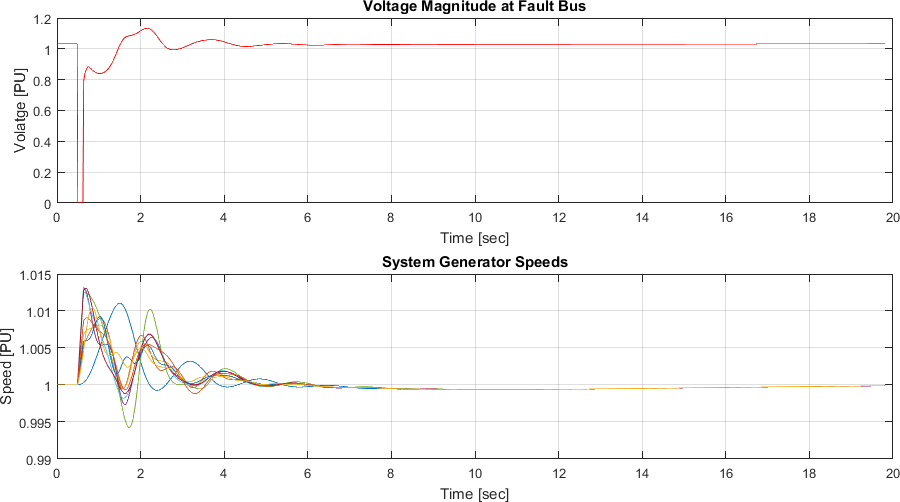
\includegraphics[width=\linewidth]{figures/hiskens/hiskensResults}
	\caption{Fault Bus Voltage and Generator Speeds from Hiskens Example.}
	\label{fig: hiskens results}
\end{figure}%\vspace{-1 em}

All PST versions (when using the same models) provide the same results, but there are differences in simulation speed and data output.
Table \ref{tab: hiskens} shows that the PST 4 simulation was roughly twice as fast as PST version 2 or 3, saved less data, and left fewer variables in the MATLAB workspace post simulation.
These improvements are likely due to the restructuring of global variables and code to remove any `all zero` data from being saved.\\

% table data for hiskens fault comparison 


\begin{table}[H]
%\resizebox{\linewidth}{!}{ % Use to resize large tables
\singlespacing
	\begin{tabular}{@{} L{1.75cm} 
	R{2cm} R{2cm}  R{2cm} @{}} 	
		\toprule % @ signs to remove extra L R space
		\footnotesize % this will affect the table font (makse it 10pt)
		\raggedright % for non justified table text
						
										
										
		PST Version	&	Simulation Time [seconds]	&	Resulting Workspace Variables	&	Saved Data Size [KB]	\\ \midrule	
		2.3	&	16.56	&	206	&	7,549	\\	
		3.1	&	16.70	&	210	&	7,548	\\	
		SETO	&	8.42	&	24	&	3,965	\\	
		4	&	7.96	&	6	&	3,974	\\	\bottomrule

													
	\end{tabular}

	\caption{PST Version Comparisons of Hiskens Example.}
	\label{tab: hiskens}
%	}%end resize box
\end{table}